\chapter{Image Acquisition and calibration}

As mentioned in the system architecture, images need to be taken simultaneously. There also needs to be two cameras due to the way the cameras are constructed, with a Bayer matrix for each pixel. At the time of inception, one could either isolate an infrared channel, or view fully RGB with separate cameras. Attempts to have both on a single camera were ineffective[].\\

\noindent
The

\section{Filters}

The blue Rosco 2008 filter is used as in Figure \ref{fig:blue_filter}, and passes only NIR within the green and red channels, as shown in Figure \ref{fig:blue_curve}.

\begin{figure}[H]
\begin{subfigure}{0.5\textwidth}
\centering
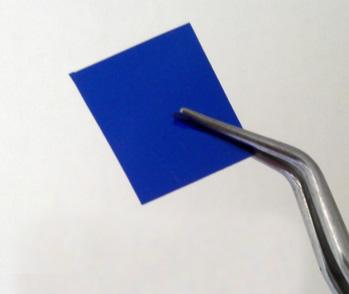
\includegraphics[scale=0.45]{images/blue_filter.jpg}
\caption{Blue Rosco 2008 filter.\\ Reproduced from \cite{blue_filter}}
\label{fig:blue_filter}
\end{subfigure}
\begin{subfigure}{0.5\textwidth}
\centering
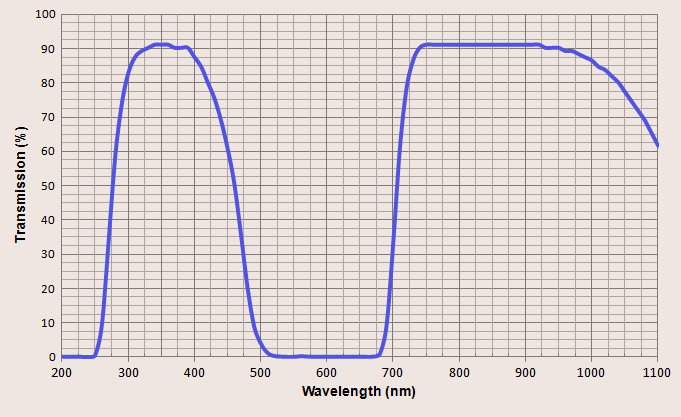
\includegraphics[scale=0.42]{images/superblueinfraredfiltercurve.png}
\caption{Blue filter transmission curve.}
\label{fig:blue_curve}
\end{subfigure}
\caption{Blue filter characteristics.\\
Reproduced from \cite{blue_curve}}
\label{fig:blue_character}
\end{figure}

\section{Camera mount}

Ripple / jello

Thus, a DC brushless motorised gimbal will not be necessary.

\section{Simultaneous triggering}

TCP triggering, scheduled triggering.

\section{Calibration}

Stereorectification